%%%%%%%%%%%%%%%%%%%%%%%%%%%%%%%%%%%%%%%%%
% a0poster Portrait Poster
% LaTeX Template
% Version 1.0 (22/06/13)
%
% The a0poster class was created by:
% Gerlinde Kettl and Matthias Weiser (tex@kettl.de)
% 
% This template has been downloaded from:
% http://www.LaTeXTemplates.com
%
% License:
% CC BY-NC-SA 3.0 (http://creativecommons.org/licenses/by-nc-sa/3.0/)
%
%%%%%%%%%%%%%%%%%%%%%%%%%%%%%%%%%%%%%%%%%

%----------------------------------------------------------------------------------------
%	PACKAGES AND OTHER DOCUMENT CONFIGURATIONS
%----------------------------------------------------------------------------------------

\documentclass[a0,portrait]{a0poster}

\usepackage{multicol} % This is so we can have multiple columns of text side-by-side
\columnsep=100pt % This is the amount of white space between the columns in the poster
\columnseprule=3pt % This is the thickness of the black line between the columns in the poster

\usepackage[svgnames]{xcolor} % Specify colors by their 'svgnames', for a full list of all colors available see here: http://www.latextemplates.com/svgnames-colors

\usepackage{times} % Use the times font
%\usepackage{palatino} % Uncomment to use the Palatino font

\usepackage{graphicx} % Required for including images
\graphicspath{{figures/}} % Location of the graphics files
\usepackage{booktabs} % Top and bottom rules for table
\usepackage[font=small,labelfont=bf]{caption} % Required for specifying captions to tables and figures
\usepackage{amsfonts, amsmath, amsthm, amssymb} % For math fonts, symbols and environments
\usepackage{wrapfig} % Allows wrapping text around tables and figures

\begin{document}

%----------------------------------------------------------------------------------------
%	POSTER HEADER 
%----------------------------------------------------------------------------------------

% The header is divided into two boxes:
% The first is 75% wide and houses the title, subtitle, names, university/organization and contact information
% The second is 25% wide and houses a logo for your university/organization or a photo of you
% The widths of these boxes can be easily edited to accommodate your content as you see fit

\begin{minipage}[b]{0.75\linewidth}
\veryHuge \color{NavyBlue} \textbf{Hand Tracking using RGB-D data} \color{Black}\\[0.5cm] % Title\Huge\textit{An Exploration of Complexity}\\[2cm] % Subtitle
\huge \textbf{Maxi We\ss \& Hanna Holderied}\\[0.5cm] % Author(s)
\huge \textbf{Hendrik Bitzmann \& Christoph Rauterberg}\\[0.5cm] % Author(s)
\huge University of G\"ottingen\\[0.4cm] % University/organization
\end{minipage}
%
\begin{minipage}[b]{0.25\linewidth}

\includegraphics[width=20cm]{logo.png}\\
\end{minipage}

\vspace{1cm} % A bit of extra whitespace between the header and poster content

\normalsize
%----------------------------------------------------------------------------------------

\begin{multicols}{2} % This is how many columns your poster will be broken into, a portrait poster is generally split into 2 columns

%----------------------------------------------------------------------------------------
%	ABSTRACT
%----------------------------------------------------------------------------------------

%\color{Navy} % Navy color for the abstract
%
%\begin{abstract}
%
%Sed fringilla tempus hendrerit. Vestibulum ante ipsum primis in faucibus orci luctus et ultrices posuere cubilia Curae; Etiam ut elit sit amet metus lobortis consequat sit amet in libero. Lorem ipsum dolor sit amet, consectetur adipiscing elit. Phasellus vel sem magna. Nunc at convallis urna. isus ante. Pellentesque condimentum dui. Etiam sagittis purus non tellus tempor volutpat. Donec et dui non massa tristique adipiscing. Quisque vestibulum eros eu. Phasellus imperdiet, tortor vitae congue bibendum, felis enim sagittis lorem, et volutpat ante orci sagittis mi. Morbi rutrum laoreet semper. Morbi accumsan enim nec tortor consectetur non commodo nisi sollicitudin. Proin sollicitudin. Pellentesque eget orci eros. Fusce ultricies, tellus et pellentesque fringilla, ante massa luctus libero, quis tristique purus urna nec nibh.
%
%\end{abstract}

%----------------------------------------------------------------------------------------
%	INTRODUCTION
%----------------------------------------------------------------------------------------

%\color{SaddleBrown} % SaddleBrown color for the introduction
%
%\section*{Introduction}
%
%Aliquam non lacus dolor, \textit{a aliquam quam} \cite{Smith:2012qr}. Cum sociis natoque penatibus et magnis dis parturient montes, nascetur ridiculus mus. Nulla in nibh mauris. Donec vel ligula nisi, a lacinia arcu. Sed mi dui, malesuada vel consectetur et, egestas porta nisi. Sed eleifend pharetra dolor, et dapibus est vulputate eu. \textbf{Integer faucibus elementum felis vitae fringilla.} In hac habitasse platea dictumst. Duis tristique rutrum nisl, nec vulputate elit porta ut. Donec sodales sollicitudin turpis sed convallis. Etiam mauris ligula, blandit adipiscing condimentum eu, dapibus pellentesque risus.
%
%\textit{Aliquam auctor}, metus id ultrices porta, risus enim cursus sapien, quis iaculis sapien tortor sed odio. Mauris ante orci, euismod vitae tincidunt eu, porta ut neque. Aenean sapien est, viverra vel lacinia nec, venenatis eu nulla. Maecenas ut nunc nibh, et tempus libero. Aenean vitae risus ante. Pellentesque condimentum dui. Etiam sagittis purus non tellus tempor volutpat. Donec et dui non massa tristique adipiscing.

%----------------------------------------------------------------------------------------
%	OBJECTIVES
%----------------------------------------------------------------------------------------

\color{DarkSlateGray} % DarkSlateGray color for the rest of the content

\Huge{\textbf{Main Objectives} }\\[0.25cm]
The main objective was to \emph{create a scene within a virtual reality} in which the user can interact with a coffe machine using his or her own hand gestures. \\
We used:
\begin{enumerate}
\item a Microsoft Kinect v2 with a infrared depth sensor, a RGB sensor and 3D motion tracking
\item A Leap Motion sensor
\end{enumerate}
\begin{center}\vspace{1cm}
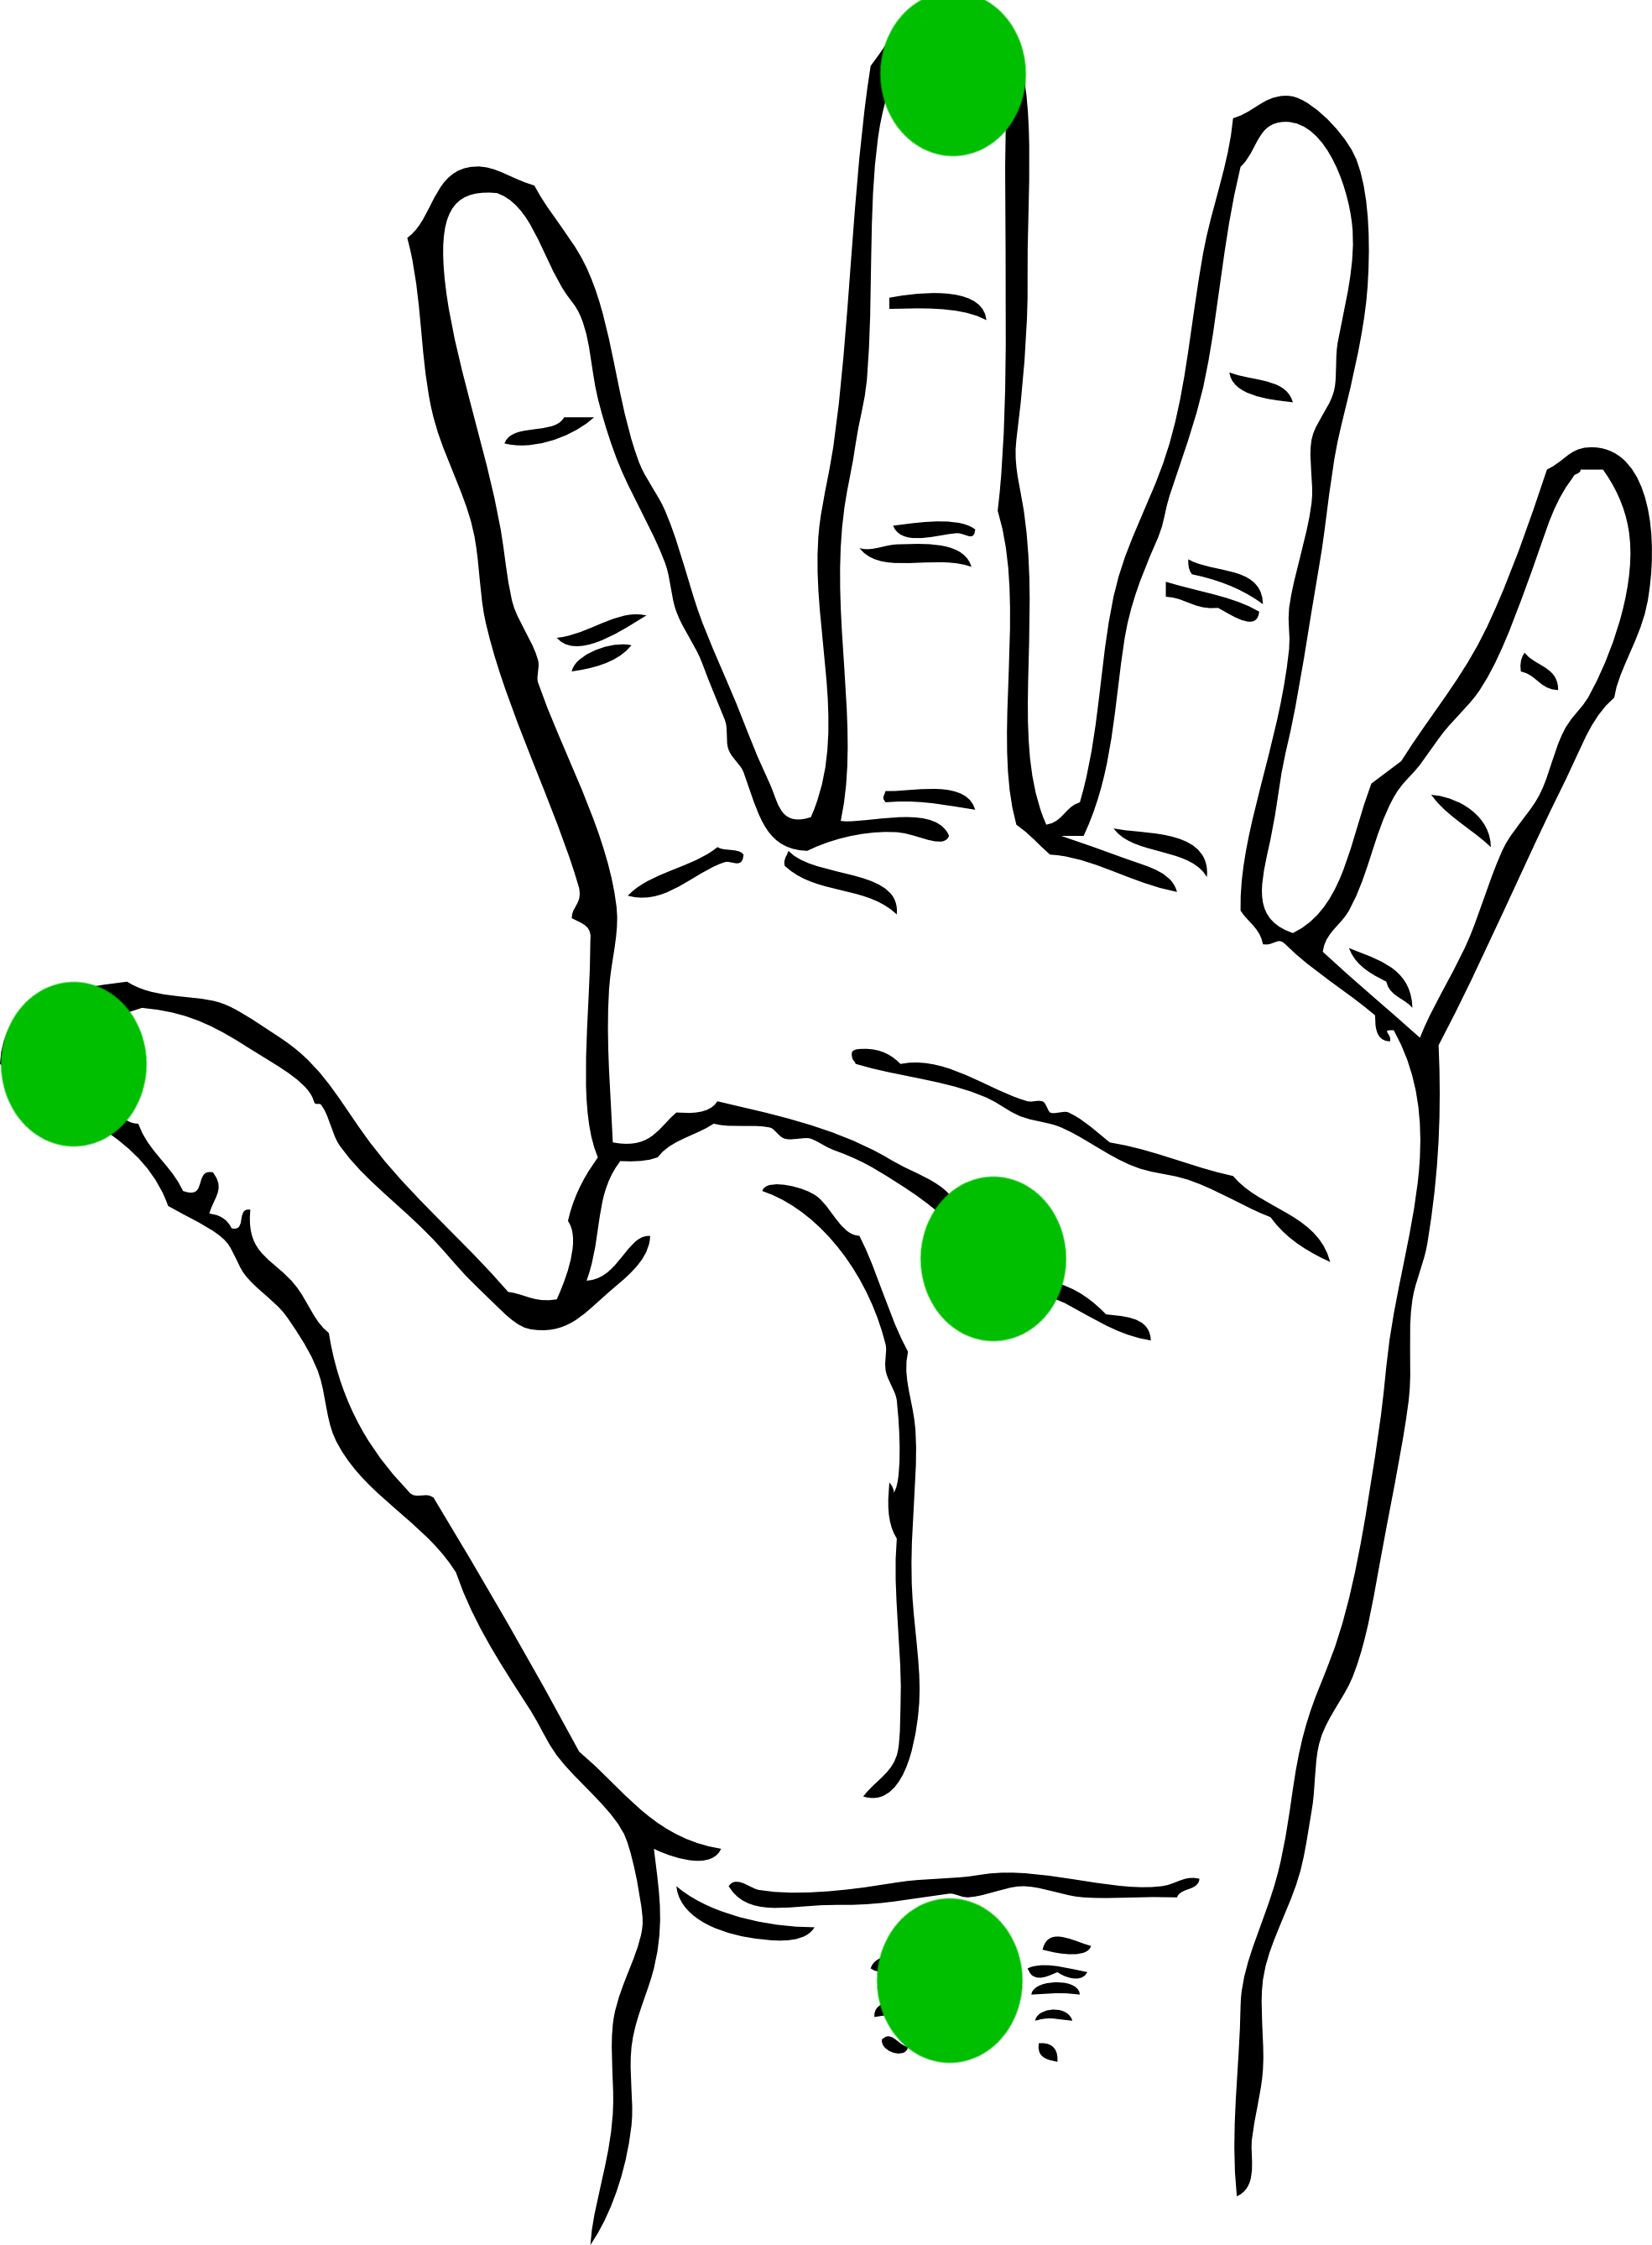
\includegraphics[width=0.5\linewidth]{./figures/palm.png}
\captionof{figure}{\color{Green} The 4 different positions we can extract from the sensors.}
\end{center}\vspace{1cm}
\color{black}
%----------------------------------------------------------------------------------------
%	MATERIALS AND METHODS
%----------------------------------------------------------------------------------------
\Huge{\textbf{Methods} }\\[0.25cm]
We are able to extract the positions of the \emph{Wrist}, the \emph{Palm}, \emph{Finger Tip} and the\emph{Thumb Tip}.\\
\cite{kinecthandonline} and \cite{joseph2016fits} show a valid approach to estimate the gesture of the hand.\\[0.1cm]
%
\Huge{\textbf{Encountered Problems} }\\[0.1cm]
In practice, \cite{kinecthandonline} proved to be unliable in bad lighting. Furthermore we experienced \emph{unstable hand orientation} which solved by computing means of positions from several frames. \\
Unfortunately, there was not enough time to fully deploy solutions such as \cite{joseph2016fits} or to fully deploy a working mesh of the two different coordinate systems provided by the Kinect and the Leap Motion Sensor.
\\[0.1cm]
%
\Huge{\textbf{Results} }\\[0.25cm]

%
In the end we were still able to provide a virtual reality in which the user can interact with a coffee machine. The user's hands are tracked and the movement is mapped into the virtual reality. Once a hand comes close to the coffee machine, the buttons will chance their color and indicate the pressing of such.
%
\begin{center}\vspace{1cm}
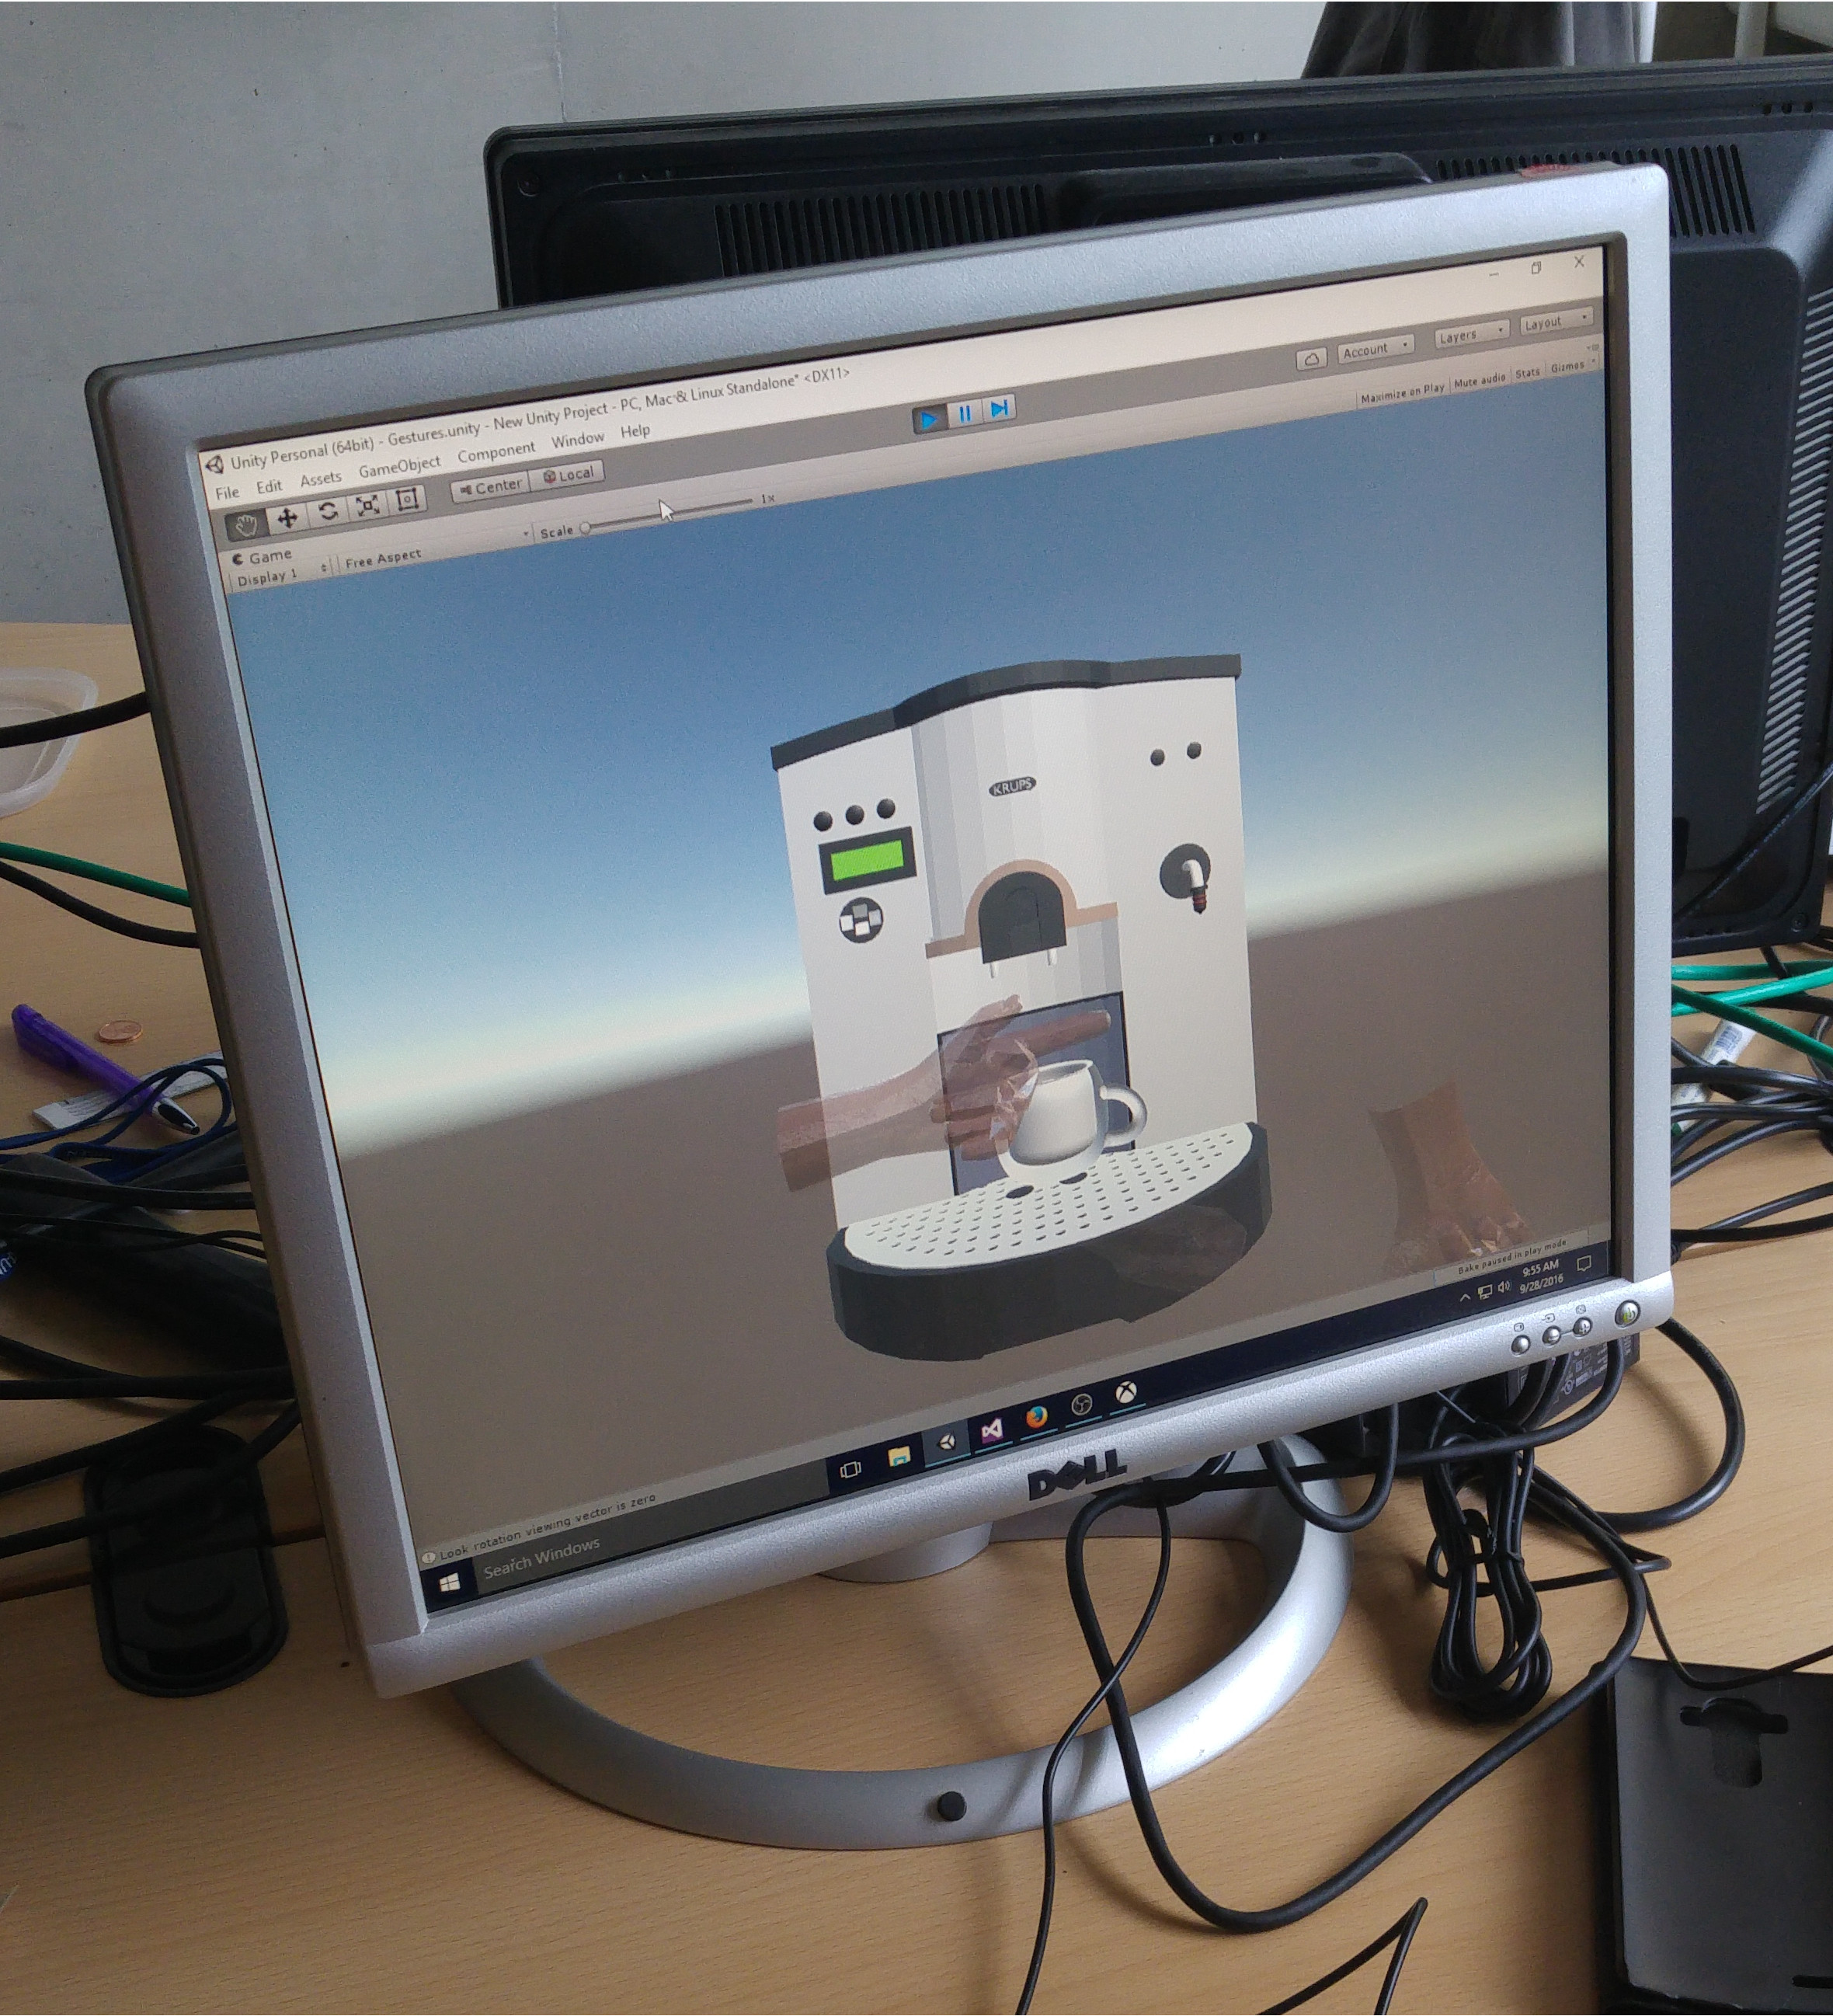
\includegraphics[width=0.5\linewidth]{./figures/vr_scene.jpg}
\captionof{figure}{\color{Green} In the virtual reality scene, the user can interact with a coffee machine using his/her own hands.}
\end{center}\vspace{1cm}

\nocite{*} % Print all references regardless of whether they were cited in the poster or not
\bibliographystyle{plain} % Plain referencing style
\bibliography{sample} % Use the example bibliography file sample.bib

%----------------------------------------------------------------------------------------

\end{multicols}
\end{document}